% !TeX root = ../main.tex
\textbf{Supercooling Lab Research Paper - Instructions}

\textbf{**Please do not edit this tab.}

Thank you all for your participation and hard work in the lab! As we
transition to the reporting phase, please keep the following guidelines
in mind:

\begin{itemize}
\item
  It is very important that you fill in this form to participate in the
  ARC competition (We will help you complete it the day of the lab
  writing session April 2nd,
  D-105):\href{https://drive.google.com/file/d/1Ut9bQdEaYGbbIEvJomWCDojfBC1YSzDY/view?usp=sharing}{\ul{ARC\_Prix-etudiants-2025-2026\_Appel-mentionsFormulaire.pdf}}
\item
  Please try to stick to the document tab labelled with your name in
  your assigned section. It is highly encouraged that you communicate
  with the other members in the same section assigned to you. If work is
  split evenly between participants in each part, the writing process
  should be relatively short and simple.👍
\item
  We've included guiding questions in each tab to help you get started.
  We colour-coded the questions to facilitate the splitting of the work.
  😊 However, please feel free to include any other observations or data
  points you feel are pertinent to the research!
\item
  \textbf{Research \& citations}: For sections requiring external
  literature, you can cite your credible academic sources in APA format.
  For help with formatting, you can refer to the
  \href{https://owl.purdue.edu/owl/research_and_citation/apa_style/apa_formatting_and_style_guide/general_format.html}{\ul{Purdue
  OWL APA Guide}}
\item
  Please note that the \textbf{Abstract} and \textbf{Conclusion} can
  only be finalized toward the end of the writing process as they
  require a complete analysis of our final results.
\end{itemize}

Keep in mind the MRT execs are planning a writing session soon during AP
(Thursday, April 2nd, D-105) so you can discuss with others, and we can
assist you in the finalization of your parts. 👍👍👍 We will be giving
out free gifts as well so please do come.

\textbf{Here are some pertinent links!}

\begin{itemize}
\item
  \href{https://docs.google.com/document/d/1_lrn-yNQTnDbAu8eqkT399SBtqj81q0VHHypbD5RuBQ/edit?usp=sharing}{\ul{Lab
  Member Handout Sheet}}
\item
  \href{https://drive.google.com/drive/folders/1HfUY64YCwoHetagSDpJOahoH-zSswrbs?usp=drive_link}{\ul{Initial
  Sample Pictures}}
\item
  \href{https://drive.google.com/drive/folders/1YSVa-CDu4g39CmCwvr0QcoKk0oyX-Gw9?usp=drive_link}{\ul{Ice-Water
  Bath Pictures}}
\item
  \href{https://drive.google.com/drive/folders/1hbAqyZgXMqdLH1_UBrjk5hroIpjT1320?usp=drive_link}{\ul{Acetone-Dry-Ice
  Pictures}}
\item
  \href{https://drive.google.com/drive/folders/1ZHALieRmtOkKvx9nMNw6_dSi68EbCrts?usp=drive_link}{\ul{Data
  Sheet (quantitative and qualitative data)}}
\item
  \href{https://drive.google.com/file/d/1pMFC6koPDrH5SM0JLRMNXgy3zwWQ-KXk/view?usp=sharing}{\ul{Scientific
  Writing Workshop Slides}} (from guest speaker Elizabeth Teel!)
\end{itemize}

\textbf{Some gentle reminders:}

\begin{itemize}
\item
  Please avoid editing other people's content without their permission.
  (We have access to the history 😁 )
\item
  If you would like to change sections, please MIO Nicolas Huni on
  \textbf{omnivox,} let him know which consenting participant you would
  like to exchange sections with and proceed with the request after
  receiving approval.
\item
  If you have any questions about format and content, feel free to
  contact us through the designated
  \href{https://discord.gg/PJDX7c8V}{\ul{Supercooling Discord Channel}}.
\end{itemize}

\textbf{Tips for scientific writing} (from guest speaker Elizabeth
Teel's slides)\textbf{:}

\begin{itemize}
\item
  How do I start?

  \begin{itemize}
  \item
    Outline or organize your thoughts.
  \item
    Just write. Don't worry about formatting, organization, citations,
    word choice, etc.
  \item
    Go back and critically edit.
  \item
    Add citations and format the document as needed.
  \end{itemize}
\item
  Words:

  \begin{itemize}
  \item
    Reduce dead weight words and phrases.
  \item
    Cut, cut, cut; remove unnecessary or redundant words.
  \item
    Be specific/precise with your words.
  \end{itemize}
\item
  Sentences:

  \begin{itemize}
  \item
    Use Active Voice: subject + verb + object (SVO).
  \item
    Use strong verbs and avoid turning verbs into nouns.
  \item
    Eliminate contractions and negative constructions.
  \end{itemize}
\end{itemize}

Introduction

\textbf{Introduction}

\textbf{Guiding Questions:}

\textbf{(Please do not modify these questions or write on this tab.
Please write in your designated tab)}

\begin{itemize}
\item
  Background:

  \begin{itemize}
  \item
    What is supercooling?
  \item
    Real-life uses?
  \item
    Warnings, precautions: (acetone dissolves plastic and styrofoam vs
    dry ice)
  \end{itemize}
\item
  Introduction to Problem:

  \begin{itemize}
  \item
    What is the role of supercooling in the preservation of fruits?
  \item
    What problem would it be solving about fruit preservation right now
    and how would it solve it?
  \item
    Provide known facts and/or statistics to establish the significance
    of the problem
  \end{itemize}
\end{itemize}

Yuechen Ma

The supercooled state is reached when a liquid's temperature is lowered
below its freezing point without observing solidification of the
substance. This process is the science behind cryopreservation,
meteorology, and certain medical therapy. Scientists use supercooling to
preserve biological samples, including blood, cells, organs, and
consumables. The supercooled state is thermodynamically unstable but is
maintained as a substance's molecular arrangement allows crystallization
only when triggered.

Narrowing the lens to the dietary aspect, previous studies show that
traditional freezing is inefficient for foods with high water content,
such as fruits and vegetables, as water expands when temperature is
lowered below 4 degrees celcius and forms crystals that eventually
rupture cell walls. Once the fruit thaws, the internal structure is
damaged and leaves the sample with texture, hydration, and nutrition
loss. In addition, common refrigeration only delays food decay for a
short period of time. In contrast, supercooling was viewed as a
potential to extend fruits' shelf life while minimizing structural
damage. By extension, efficient usage of tools will bring significant
change in the economic sphere, lowering post-harvest loss, which was
reported to make up 20-40\% of fruits and vegetables by the Food and
Agriculture Organization (FAO).

The execution of supercooling requires extreme caution. Acetone is
highly flammable and chemically reactive with most plastics and
styrofoam, necessitating the usage of stainless steel or heavy-duty
glass such as Pyrex as experimental containers. The manipulation of dry
ice should be done with protective gear and within a fume hood. Direct
skin contact can cause thermal burns and poor ventilation leads to
inhalation of excess CO\textsubscript{2} as dry ice sublimates into gas.

Eliana Gasparrini

Other research in supercooling has been done for agricultural purposes.
Currently, in Canada, late spring frosts often kill off crops once to
twice a year. Some examples of the fruits are apples, apricots,
blackberries, blueberries, cherries, grapes, peaches, pears, plums and
raspberries. Both the fruit and the flowers can sustain frost injuries
if the temperature is lower than their ability to supercool (Palonen \&
Buszard, 1997). In the Okanagan valley, a Canadian region that produces
a lot of wine grapes, climate change is worsening the extreme
temperatures that cause grapes to exceed their supercooling capacity.
Research also shows that the same goes for sweet cherries and apples
(Quamme et al., 2010).

The Australian Journal of Grape and Wine Research published an article
examining the supercooling temperature of 43 different genotypes of
grapes, with the goal of seeing which ones would be most useful to
incorporate into future hybrids. Grapes that supercool at lower
temperatures are said to have more cold hardiness, and these ones will
be selected to be part of future hybrid species since they improve the
new species' early winter hardiness (Londo \& Kovaleski, 2019). This can
be used for other fruit species as well. The ability of fruits to
supercool is influenced by their geographical distribution, so by
breeding hardier species with ones that freeze more easily but taste
better, the hybrid crops will be able to grow in colder environments
while still retaining characteristics of the more commonly eaten
varieties. Future research in how to genetically engineer the species
for higher cold hardiness can allow, for example, an eventual way to
grow stone fruits such as peaches higher north than is currently
possible (Quamme, 1991). This eliminates some of the transportation
steps in the current supply chain, which is beneficial for the
environmental impact, the taste, and the price of the product.

To add to the preservation methods section (second paragraph on previous
tab):

Alternating magnetic fields (AMFs) have also been shown to help with
grapes being preserved at a supercooling temperature. They lower the ice
nucleation temperature, which may be thanks to the vibration of the
atoms which makes it harder for ice to crystallize and therefore reduces
freezing injuries in grapes (Jiang et al., 2025). Using magnetic fields,
as well as electric fields, to delay ice nucleation is an important path
for future research as the mechanism in which it stops crystal formation
is still largely unknown (Kang et al., 2020).

1. Sources

\textbf{Sources:\\
}

\textbf{All facts that are stated that were not discovered by you should
be cited in the report. All citations should have a corresponding
bibliography entry in this section.}

\begin{quote}
Atta U Rehman Chachar. ``Reducing Post-Harvest Losses for Food
Security.'' \emph{Agrieconomist}, The AgEcon Frontiers, 12 May 2025,
\href{https://www.agrieconomist.com/reducing-post-harvest-losses-for-food-security}{\ul{Reducing
Post-Harvest Losses for Food Security \textbar{} The Agricultural
Economist}}.

\hl{Biology Insights. "What is Supercooling and How Does This Phenomenon
Work?" \emph{Biology Insights}, 25 Aug. 2025,}
\href{https://biologyinsights.com/what-is-supercooling-and-how-does-this-phenomenon-work/}{\ul{What
Is Supercooling and How Does This Phenomenon Work? - Biology Insights}}.

Food and Agriculture Organization. ``Prevention of post-harvest food
losses fruits, vegetables and root crops a training manual.'' \emph{Food
and Agriculture Organization of the United Nations}, 01 Jan 1989,
\href{https://www.fao.org/4/T0073E/T0073E01.htm}{\ul{Prevention of
post-harvest food losses fruits, vegetables and root crops a training
manual - Foreword-Preface-Introduction-Nutrition and fresh
produce-Pre-harvest factors in produce marketing-Perishability and
produce losses}}.

Lin, Hengxun, et al. ``The importance of supercooled stability for food
during supercooling preservation: a review of mechanisms, influencing
factors, and control methods.'' \emph{Taylor \& Francis Online}, 05 Sep
2023,
\href{https://www.tandfonline.com/doi/abs/10.1080/10408398.2023.2248515}{\ul{The
importance of supercooled stability for food during supercooling
preservation: a review of mechanisms, influencing factors, and control
methods: Critical Reviews in Food Science and Nutrition: Vol 64, No
33}}.
\end{quote}

(As cited in-text on previous tab: )

\begin{quote}
Jiang, H., Zhao, S., Li, S., Wang, H., Han, X., \& Guan, W. (2025).
Effect of alternating magnetic field on ice crystal nucleation and its
application for near-freezing temperature storage of grapes.
\emph{Journal of Future Foods}, \emph{5}(2), 193--199.
https://doi.org/10.1016/j.jfutfo.2024.05.008

Kang, T., You, Y., \& Jun, S. (2020). Supercooling preservation
technology in food and biological samples: a review focused on electric
and magnetic field applications. In \emph{Food Science and
Biotechnology} (Vol. 29, Number 3, pp. 303--321). The Korean Society of
Food Science and Technology. https://doi.org/10.1007/s10068-020-00750-6

Londo, J. P., \& Kovaleski, A. P. (2019). Deconstructing cold hardiness:
variation in supercooling ability and chilling requirements in the wild
grapevine Vitis riparia. \emph{Australian Journal of Grape and Wine
Research}, \emph{25}(3), 276--285. https://doi.org/10.1111/ajgw.12389

Palonen, P., \& Buszard, D. (1997). Current state of cold hardiness
research on fruit crops. \emph{Canadian Journal of Plant Science},
\emph{77}(3), 399--420. https://doi.org/10.4141/P96-013

Quamme, H. A. (1991). Application of Thermal Analysis to Breeding Fruit
Crops for Increased Cold Hardiness. \emph{HortScience}, \emph{26}(5),
513--517. https://doi.org/10.21273/HORTSCI.26.5.513

Quamme, H. A., Cannon, A. J., Neilsen, D., Caprio, J. M., \& Taylor, W.
G. (2010). The potential impact of climate change on the occurrence of
winter freeze events in six fruit crops grown in the Okanagan Valley.
\emph{Canadian Journal of Plant Science}, \emph{90}(1), 85--93.
https://doi.org/10.4141/CJPS09042
\end{quote}

Objective + Variables

\textbf{Objective and Variables}

\textbf{Guiding Questions:}

\textbf{(Please do not modify these questions or write on this tab.
Please write in your designated tab)}

\begin{itemize}
\item
  What was the objective?
\end{itemize}

\begin{itemize}
\item
  Variables:

  \begin{itemize}
  \item
    What changed between each trial? I.e. Independant, dependant
  \item
    What are the control groups?
  \item
    What were the different fruits we tried supercooling and why?
  \item
    What are the different techniques that we used for
    freezing/supercooling?
  \end{itemize}
\end{itemize}

Erqi Wei

The aim of this experiment was to determine how the cooling of grapes
and apples through ice-water brine bath and the cooling of grapes
through dry-acetone solution impact the fruits' physical properties. The
following physical properties of the fruits are measured:

\begin{itemize}
\item
  Change of mass (g)
\item
  Texture
\item
  Microscopic structure
\end{itemize}

Methodology

\textbf{Methodology}

\textbf{Guiding Questions:}

\textbf{(Please do not modify these questions or write on this tab.
Please write in your designated tab)}

\begin{itemize}
\item
  What were the materials and instruments we used and why? Please use
  full sentences.
\item
  Protocol:

  \begin{itemize}
  \item
    How the data were collected
  \item
    Where the data were collected
  \item
    When the data were collected (period was completed over)
  \item
    Order the data were collected in
  \item
    Who collected the data
  \end{itemize}
\item
  Were there any sources of error that we could not control/would be
  hard to control?
\item
  Were there any precautions?
\end{itemize}

Victor Zhan

The sample fruits of the experiment consisted of store-bought seedless
green grapes and Red Prince apples, which have freezing points of around
-2.2 °C and -1.7 °C respectively (Zhao et al., 2025 ; World Food
Logistics Organization {[}WFLO{]}, 2018). The fruits were cut into small
rectangular prisms of roughly 2.5 x 1.0 x 0.5 cm beforehand to speed up
the supercooling process. The weight (g) of the samples was measured and
their texture was qualitatively determined before the supercooling to
serve as baselines for comparison. The fruit samples were placed in
air-evacuated ziploc bags to isolate them from the acetone and ice-water
mixture used for the fast and slow supercooling trials respectively. The
fruit samples were submerged in an -30 °C acetone filled beaker cooled
by dry ice for the instant flash-freezing trials and in a -8 °C mixture
of water, crushed ice and salt for the slow supercooling trials. The
samples were allowed to freeze completely and the exact freezing points
of the samples for the trials were determined using an infrared
thermometer. The samples were thawed at room temperature and their
post-thaw weights and textures were determined. The thawed and unfrozen
control samples were cut into 0.5-mm-thick slivers using a sharp razor
blade for microscopic analysis. A standard lab microscope was used to
analyze the cellular structure of the unfrozen control samples, the
thawed slowly supercooled samples as well as the thawed instant
flash-frozen samples.

Potential errors

\begin{itemize}
\item
  Pesticides, GMO or similar factor depending on the fruits
\item
  The introduction of more bacteria acting as nucleation sites through
  contamination from outside sources
\item
  Potential differences between individual grapes and different regions
  of the same apple (maybe slight difference in sugar/water
  concentration between part of apple closer to base and closer to stem)
\item
  Very hard to visually determine the exact moment the apple sample
  freezes due to opacity
\end{itemize}

\textbf{Notes}

\begin{itemize}
\item
  We can specify what variety (Honeycrisp, Gala, etc.) of apple and
  grapes were used if we have the info
\item
  The dimensions of the fruit prism are just really rough estimates if
  excecs have real dimension could put them instead
\end{itemize}

Ahjin Joo

The experiment was divided into two parts: supercooling of apples and
grapes and flash-freezing of the same fruits. For each method,
temperature, mass before and after freezing, texture, and microscopic
damage after thawing were recorded.

First, the fruits were cut into three pieces each. The initial texture
of each sample was observed, and the mass of each piece was measured in
grams. In other words, a total of six masses were recorded. The first
batch of fruits served as the control, the second batch was used for the
acetone-dry ice bath, and the third batch was used for the ice-water
bath.

For the ice-water bath, the fruit samples were placed in plastic bags,
and excess air was removed. The samples were then submerged in the
cooling bath and left undisturbed for 15-20 minutes. The temperature was
monitored, and the temperature immediately before freezing began was
recorded. The samples were allowed to freeze completely, then thawed at
room temperature. After thawing, the final mass of each sample was
measured, and mass loss was calculated. Changes in physical texture were
observed, and the samples were examined under a microscope while images
were taken at magnifications of 4x, 10x, and 40x.

For the rapid freezing method, a dry ice and acetone bath was prepared
in a fume hood and allowed to reach approximately -30 degrees Celsius.
Fruit samples were placed in test tubes and fully submerged in the bath.
The temperature was monitored until freezing began, and the freezing
temperature was recorded. The samples were allowed to freeze completely
and were then thawed at room temperature. After thawing, the same
procedures were followed: the final mass was measured, mass loss was
calculated, texture changes were observed, and microscopic images were
taken.

Savva Zosimov

Fruit samples of apple and grape were removed from storage and control
samples were taken out of their containers. The initial texture of each
sample was examined visually and manually, and these observations were
recorded to establish a baseline for later comparison. An ice-water bath
was prepared. Water (100 mL) was placed into a container, and 50g of
NaCl was added, as well as a magnetic stir bar to maintain uniform
cooling throughout the bath. Ice was introduced in increments beginning
with 50g until the mixture reached -8℃. Fruit samples were weighed on an
electronic balance, and their initial masses were recorded. Each sample
was sealed inside a plastic bag and fully submerged in the brine bath.
The samples were cooled for 15-20 min and their temperatures were
periodically monitored using a non-contact infrared thermometer. The
bath was not disturbed during cooling to prevent ice formation.
Supercooling was identified when the temperature of a sample fell below
0℃ while the fruit remained unfrozen (no ice formed) and the temperature
was recorded. Samples were then allowed to freeze completely before
being removed and thawed at room temperature. Once thawed, samples were
reweighed, mass loss was calculated, and post-thaw texture
characteristics were documented. Finally, photographs of thawed samples
were taken.

A dry ice - acetone bath was prepared inside a fume hood: dry ice was
placed into a Styrofoam container and a large beaker was placed within
it. Acetone (5L) was poured into the beaker, and the mixture was allowed
to cool to -30℃. New fruit samples were weighed and their masses were
recorded. Each sample was placed into a dry test tube, which was
positioned upright in the acetone bath so that the fruit-containing
portion was fully submerged. Using an infrared thermometer, sample
temperatures were monitored continuously and the temperature at which
solidification began was recorded. The samples were then frozen
completely, removed from the bath, and thawed at room temperature. Final
masses were measured, mass loss was calculated, post-thaw
characteristics were recorded, and photographs of thawed samples were
taken.

Fresh fruit samples that had not undergone freezing were sliced into
approximately 0.5mm slivers using a razor blade. Each sliver was placed
on a glass microscope slide and positioned on the microscope stage.
Magnification was increased incrementally, photographs of samples were
taken at these magnifications, and the cellular structure of fresh
samples were described. The same procedure was repeated for thawed
samples from both cooling methods, ice - water bath and dry ice -
acetone bath.

Sources of error included reading inaccuracy from the infrared
thermometer, the possibility of uneven cooling within the baths and
accidental bath disturbances that may have triggered premature ice
forming. Natural variation in fruit size and ripeness may have affected
freezing behavior and mass loss (ex: different cultivars?). Small losses
of juice during handling or residual moisture on samples could have
influenced mass measurements. In microscopic analysis, inconsistent
slice thickness may have introduced variability.

2. Sources

\textbf{Sources:\\
}

\textbf{All facts that are stated that were not discovered by you should
be cited in the report. All citations should have a corresponding
bibliography entry in this section.}

\begin{quote}
Zhao, S., Liu, J., Jiang, H., Yang, X., Guan, W., Liu, B., Lv, Z., \&
Chen, C. (2025). Study on electrostatic field assisted freezing
temperature storage of grapes. \emph{Journal of Food Engineering},
\emph{394}, 112527.
\href{https://doi.org/10.1016/j.jfoodeng.2025.112527}{\ul{https://doi.org/10.1016/j.jfoodeng.2025.112527}}

World Food Logistics Organization. (2018). \emph{WFLO commodity storage
manual apples, controlled atmosphere storage 1}. Apples.
\href{https://www.gcca.org/legacy-system/WFLO-Commodity-Storage-Manual-2018Apples_Controlled_Atmosphere\%5B1\%5D_0.pdf}{\ul{https://www.gcca.org/legacy-system/WFLO-Commodity-Storage-Manual-2018Apples\_Controlled\_Atmosphere\%5B1\%5D\_0.pdf}}
\end{quote}

Results

\textbf{Results}

\textbf{(Please do not modify these questions or write on this tab.
Please write in your designated tab)}

\textbf{Useful links:}

\begin{itemize}
\item
  \href{https://drive.google.com/drive/folders/1HfUY64YCwoHetagSDpJOahoH-zSswrbs?usp=drive_link}{\ul{Initial
  Sample Pictures}}
\item
  \href{https://drive.google.com/drive/folders/1YSVa-CDu4g39CmCwvr0QcoKk0oyX-Gw9?usp=drive_link}{\ul{Ice-Water
  Bath Pictures}}
\item
  \href{https://drive.google.com/drive/folders/1hbAqyZgXMqdLH1_UBrjk5hroIpjT1320?usp=drive_link}{\ul{Acetone-Dry-Ice
  Pictures}}
\item
  \href{https://drive.google.com/drive/folders/1ZHALieRmtOkKvx9nMNw6_dSi68EbCrts?usp=drive_link}{\ul{Data
  Sheet (quantitative and qualitative data)}}
\end{itemize}

The results section describes the main study findings provided
\emph{without interpretation}.

You can use graphs and tables to communicate the information recorded in
the lab visually. (Make sure to label the axis and include appropriate
titles!)

Joanne Yu

For more detailed statistical analysis of mass loss results, see
\href{https://marianopolis-my.sharepoint.com/:x:/p/2530377/IQDTWQmckaVSRoRBsjZPNODiAcFLZOoIPYYXYop16nXLMGU?e=eLPE3d}{\ul{Graphs\_MRT
Lab Results.xlsx}}.

\includegraphics[width=5.94271in,height=3.80943in]{media/image5.png}

\textbf{Note:} 2 outlier mass values were excluded from all mass loss
calculations.

\ul{(TO REMOVE in the final version of the report after the Analysis
section is completed):}

\begin{itemize}
\item
  Generally, less mass loss for apple vs. grape, less mass loss for
  acetone vs. ice-bath (based on median)
\item
  No clear distinction between ice-bath and acetone
\item
  Apple - Ice-Bath most concentrated, Apple - Acetone most dispersed
  (see standard deviation in data tables)
\end{itemize}

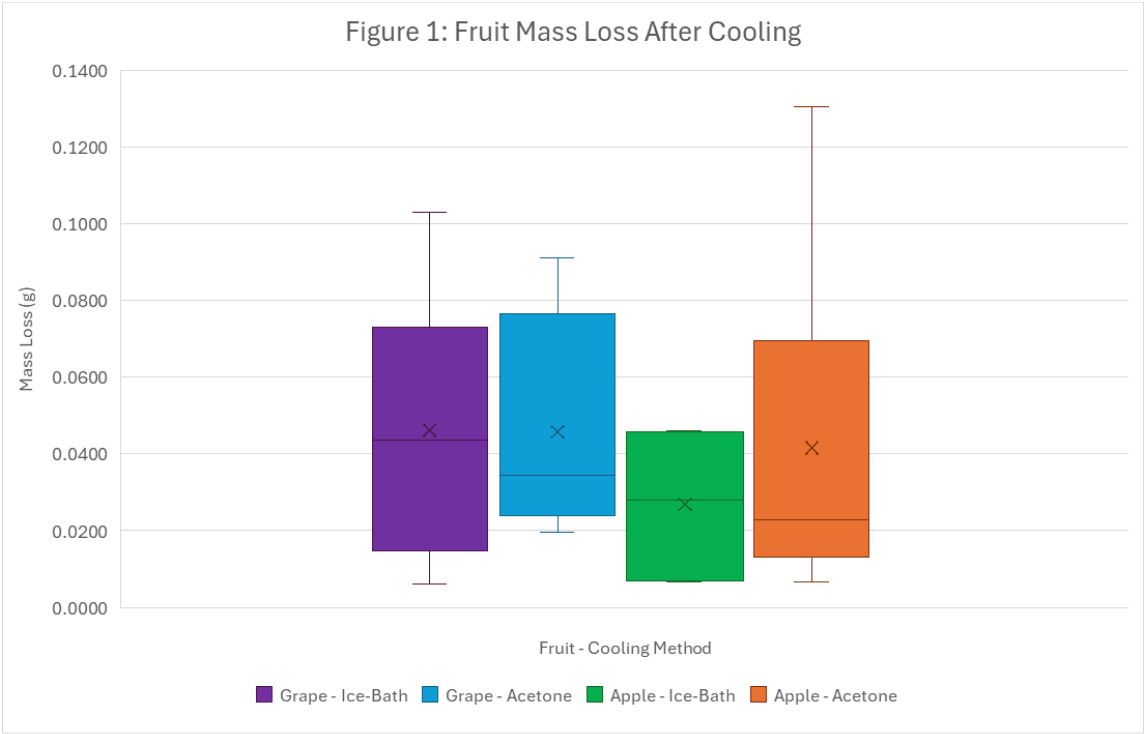
\includegraphics[width=6.10938in,height=4.35467in]{media/image1.png}

\textbf{Note:} 2 outlier temperature values (with corresponding mass
values) were excluded from all mass loss relative to freezing point
calculations.

\ul{(TO REMOVE):}

\begin{itemize}
\item
  No clear (linear) relations
\item
  Different mass loss results observed for the same temperature (ex:
  -15.0) = no relation
\item
  Acetone reaches lower temperatures than ice-bath
\item
  Minimum mass loss results for ice-bath are lower
\end{itemize}

Table 1: Freezing Point For Minimum Fruit Mass Loss

{\def\LTcaptype{none} % do not increment counter
\begin{longtable}[]{@{}
  >{\raggedright\arraybackslash}p{(\linewidth - 6\tabcolsep) * \real{0.0949}}
  >{\raggedright\arraybackslash}p{(\linewidth - 6\tabcolsep) * \real{0.2283}}
  >{\raggedright\arraybackslash}p{(\linewidth - 6\tabcolsep) * \real{0.3006}}
  >{\raggedright\arraybackslash}p{(\linewidth - 6\tabcolsep) * \real{0.2412}}@{}}
\toprule\noalign{}
\begin{minipage}[b]{\linewidth}\raggedright
Fruit
\end{minipage} & \begin{minipage}[b]{\linewidth}\raggedright
Cooling Method
\end{minipage} & \begin{minipage}[b]{\linewidth}\raggedright
Minimum Mass Loss (g)
\end{minipage} & \begin{minipage}[b]{\linewidth}\raggedright
Freezing Point (°C)
\end{minipage} \\
\multirow{2}{*}{\begin{minipage}[b]{\linewidth}\raggedright
Grape
\end{minipage}} & \begin{minipage}[b]{\linewidth}\raggedright
Ice-Water Bath
\end{minipage} & \begin{minipage}[b]{\linewidth}\raggedright
0.0061
\end{minipage} & \begin{minipage}[b]{\linewidth}\raggedright
-4.1
\end{minipage} \\
& \begin{minipage}[b]{\linewidth}\raggedright
Acetone-Dry Ice
\end{minipage} & \begin{minipage}[b]{\linewidth}\raggedright
0.0196
\end{minipage} & \begin{minipage}[b]{\linewidth}\raggedright
-15.0
\end{minipage} \\
\multirow{2}{*}{\begin{minipage}[b]{\linewidth}\raggedright
Apple
\end{minipage}} & \begin{minipage}[b]{\linewidth}\raggedright
Ice-Water Bath
\end{minipage} & \begin{minipage}[b]{\linewidth}\raggedright
0.0067
\end{minipage} & \begin{minipage}[b]{\linewidth}\raggedright
-4.0
\end{minipage} \\
& \begin{minipage}[b]{\linewidth}\raggedright
Acetone-Dry Ice
\end{minipage} & \begin{minipage}[b]{\linewidth}\raggedright
0.0108
\end{minipage} & \begin{minipage}[b]{\linewidth}\raggedright
-12.0
\end{minipage} \\
\midrule\noalign{}
\endhead
\bottomrule\noalign{}
\endlastfoot
\end{longtable}
}

Figures 3-6: Specific Fruit Mass Loss Relative To Freezing Point And
Cooling
Method\includegraphics[width=3.75488in,height=2.52815in]{media/image3.png}\includegraphics[width=3.73438in,height=2.52848in]{media/image7.png}

\includegraphics[width=3.75in,height=2.54717in]{media/image6.png}\includegraphics[width=3.73958in,height=2.53125in]{media/image4.png}

\ul{(TO REMOVE):}

\begin{itemize}
\item
  NOTE: Individual graphs/trendlines (Figures 3-6) can be removed or
  combined depending on how relevant they are for the analysis
\end{itemize}

\begin{itemize}
\item
  Weak linear relations (\textasciitilde none)
\item
  Negative trend line for ice-bath, positive trend line for acetone
  -\textgreater{} least mass loss for ice-bath = warmer temp, least mass
  loss for acetone = colder temp
\end{itemize}

Table 2: Confidence Interval By Fruit And Cooling Method

{\def\LTcaptype{none} % do not increment counter
\begin{longtable}[]{@{}
  >{\raggedright\arraybackslash}p{(\linewidth - 2\tabcolsep) * \real{0.3337}}
  >{\raggedright\arraybackslash}p{(\linewidth - 2\tabcolsep) * \real{0.3144}}@{}}
\toprule\noalign{}
\begin{minipage}[b]{\linewidth}\raggedright
Fruit - Cooling Method
\end{minipage} & \begin{minipage}[b]{\linewidth}\raggedright
Confidence Interval (95) (g)
\end{minipage} \\
\begin{minipage}[b]{\linewidth}\raggedright
Grape - Ice-Water Bath
\end{minipage} & \begin{minipage}[b]{\linewidth}\raggedright
{[}0.0186 -- 0.0738{]}
\end{minipage} \\
\begin{minipage}[b]{\linewidth}\raggedright
Grape - Acetone-Dry Ice
\end{minipage} & \begin{minipage}[b]{\linewidth}\raggedright
{[}0.0261 -- 0.0655{]}
\end{minipage} \\
\begin{minipage}[b]{\linewidth}\raggedright
Apple - Ice-Water Bath
\end{minipage} & \begin{minipage}[b]{\linewidth}\raggedright
{[}0.0122 -- 0.0416{]}
\end{minipage} \\
\begin{minipage}[b]{\linewidth}\raggedright
Apple - Acetone-Dry Ice
\end{minipage} & \begin{minipage}[b]{\linewidth}\raggedright
{[}0.0120 -- 0.0712{]}
\end{minipage} \\
\midrule\noalign{}
\endhead
\bottomrule\noalign{}
\endlastfoot
\end{longtable}
}

Table 3: Confidence Interval By Data Group

{\def\LTcaptype{none} % do not increment counter
\begin{longtable}[]{@{}
  >{\raggedright\arraybackslash}p{(\linewidth - 2\tabcolsep) * \real{0.3353}}
  >{\raggedright\arraybackslash}p{(\linewidth - 2\tabcolsep) * \real{0.3160}}@{}}
\toprule\noalign{}
\begin{minipage}[b]{\linewidth}\raggedright
Data Group
\end{minipage} & \begin{minipage}[b]{\linewidth}\raggedright
Confidence Interval (95) (g)
\end{minipage} \\
\begin{minipage}[b]{\linewidth}\raggedright
Grape
\end{minipage} & \begin{minipage}[b]{\linewidth}\raggedright
{[}0.0304 -- 0.0616{]}
\end{minipage} \\
\begin{minipage}[b]{\linewidth}\raggedright
Apple
\end{minipage} & \begin{minipage}[b]{\linewidth}\raggedright
{[}0.0174 -- 0.0532{]}
\end{minipage} \\
\begin{minipage}[b]{\linewidth}\raggedright
Ice-Water Bath
\end{minipage} & \begin{minipage}[b]{\linewidth}\raggedright
{[}0.0205 -- 0.0525{]}
\end{minipage} \\
\begin{minipage}[b]{\linewidth}\raggedright
Acetone-Dry Ice
\end{minipage} & \begin{minipage}[b]{\linewidth}\raggedright
{[}0.0265 -- 0.0609{]}
\end{minipage} \\
\begin{minipage}[b]{\linewidth}\raggedright
All
\end{minipage} & \begin{minipage}[b]{\linewidth}\raggedright
{[}0.0288 -- 0.0524{]}
\end{minipage} \\
\midrule\noalign{}
\endhead
\bottomrule\noalign{}
\endlastfoot
\end{longtable}
}

Source: Online Confidence Interval Calculator
(\href{https://www.calculator.net/confidence-interval-calculator.html}{\ul{https://www.calculator.net/confidence-interval-calculator.html}})

Justin Zheng

{\def\LTcaptype{none} % do not increment counter
\begin{longtable}[]{@{}
  >{\raggedright\arraybackslash}p{(\linewidth - 8\tabcolsep) * \real{0.1664}}
  >{\raggedright\arraybackslash}p{(\linewidth - 8\tabcolsep) * \real{0.1152}}
  >{\raggedright\arraybackslash}p{(\linewidth - 8\tabcolsep) * \real{0.2544}}
  >{\raggedright\arraybackslash}p{(\linewidth - 8\tabcolsep) * \real{0.2384}}
  >{\raggedright\arraybackslash}p{(\linewidth - 8\tabcolsep) * \real{0.2256}}@{}}
\toprule\noalign{}
\begin{minipage}[b]{\linewidth}\raggedright
Method
\end{minipage} & \begin{minipage}[b]{\linewidth}\raggedright
Fruit
\end{minipage} & \begin{minipage}[b]{\linewidth}\raggedright
Average temperature (°C)
\end{minipage} & \begin{minipage}[b]{\linewidth}\raggedright
Median temperature (°C)
\end{minipage} & \begin{minipage}[b]{\linewidth}\raggedright
Standard deviation (°C)
\end{minipage} \\
\begin{minipage}[b]{\linewidth}\raggedright
Ice-Water Bath
\end{minipage} & \begin{minipage}[b]{\linewidth}\raggedright
Grape
\end{minipage} & \begin{minipage}[b]{\linewidth}\raggedright
−3.29
\end{minipage} & \begin{minipage}[b]{\linewidth}\raggedright
−3.50
\end{minipage} & \begin{minipage}[b]{\linewidth}\raggedleft
2.12
\end{minipage} \\
\begin{minipage}[b]{\linewidth}\raggedright
Ice-Water Bath
\end{minipage} & \begin{minipage}[b]{\linewidth}\raggedright
Apple
\end{minipage} & \begin{minipage}[b]{\linewidth}\raggedright
−2.79
\end{minipage} & \begin{minipage}[b]{\linewidth}\raggedright
−3.10
\end{minipage} & \begin{minipage}[b]{\linewidth}\raggedleft
1.5
\end{minipage} \\
\begin{minipage}[b]{\linewidth}\raggedright
Acetone-Dry Ice
\end{minipage} & \begin{minipage}[b]{\linewidth}\raggedright
Grape
\end{minipage} & \begin{minipage}[b]{\linewidth}\raggedright
−15.03
\end{minipage} & \begin{minipage}[b]{\linewidth}\raggedright
−15.00
\end{minipage} & \begin{minipage}[b]{\linewidth}\raggedleft
4.88
\end{minipage} \\
\begin{minipage}[b]{\linewidth}\raggedright
Acetone-Dry Ice
\end{minipage} & \begin{minipage}[b]{\linewidth}\raggedright
Apple
\end{minipage} & \begin{minipage}[b]{\linewidth}\raggedright
−13.30
\end{minipage} & \begin{minipage}[b]{\linewidth}\raggedright
−14.00
\end{minipage} & \begin{minipage}[b]{\linewidth}\raggedleft
2.82
\end{minipage} \\
\midrule\noalign{}
\endhead
\bottomrule\noalign{}
\endlastfoot
\end{longtable}
}

{\def\LTcaptype{none} % do not increment counter
\begin{longtable}[]{@{}
  >{\raggedright\arraybackslash}p{(\linewidth - 8\tabcolsep) * \real{0.1648}}
  >{\raggedright\arraybackslash}p{(\linewidth - 8\tabcolsep) * \real{0.1168}}
  >{\raggedright\arraybackslash}p{(\linewidth - 8\tabcolsep) * \real{0.2544}}
  >{\raggedright\arraybackslash}p{(\linewidth - 8\tabcolsep) * \real{0.2320}}
  >{\raggedright\arraybackslash}p{(\linewidth - 8\tabcolsep) * \real{0.2320}}@{}}
\toprule\noalign{}
\begin{minipage}[b]{\linewidth}\raggedright
Method
\end{minipage} & \begin{minipage}[b]{\linewidth}\raggedright
Fruit
\end{minipage} & \begin{minipage}[b]{\linewidth}\raggedright
Average mass loss (g)
\end{minipage} & \begin{minipage}[b]{\linewidth}\raggedright
Median mass loss (g)
\end{minipage} & \begin{minipage}[b]{\linewidth}\raggedright
Standard deviation (g)
\end{minipage} \\
\begin{minipage}[b]{\linewidth}\raggedright
Ice-Water Bath
\end{minipage} & \begin{minipage}[b]{\linewidth}\raggedright
Grape
\end{minipage} & \begin{minipage}[b]{\linewidth}\raggedleft
0.0462
\end{minipage} & \begin{minipage}[b]{\linewidth}\raggedleft
0.0436
\end{minipage} & \begin{minipage}[b]{\linewidth}\raggedleft
0.0345
\end{minipage} \\
\begin{minipage}[b]{\linewidth}\raggedright
Ice-Water Bath
\end{minipage} & \begin{minipage}[b]{\linewidth}\raggedright
Apple
\end{minipage} & \begin{minipage}[b]{\linewidth}\raggedleft
0.0269
\end{minipage} & \begin{minipage}[b]{\linewidth}\raggedleft
0.028
\end{minipage} & \begin{minipage}[b]{\linewidth}\raggedleft
0.0184
\end{minipage} \\
\begin{minipage}[b]{\linewidth}\raggedright
Acetone-Dry Ice
\end{minipage} & \begin{minipage}[b]{\linewidth}\raggedright
Grape
\end{minipage} & \begin{minipage}[b]{\linewidth}\raggedleft
0.0458
\end{minipage} & \begin{minipage}[b]{\linewidth}\raggedleft
0.0345
\end{minipage} & \begin{minipage}[b]{\linewidth}\raggedleft
0.0284
\end{minipage} \\
\begin{minipage}[b]{\linewidth}\raggedright
Acetone-Dry Ice
\end{minipage} & \begin{minipage}[b]{\linewidth}\raggedright
Apple
\end{minipage} & \begin{minipage}[b]{\linewidth}\raggedleft
0.0416
\end{minipage} & \begin{minipage}[b]{\linewidth}\raggedleft
0.0227
\end{minipage} & \begin{minipage}[b]{\linewidth}\raggedleft
0.0427
\end{minipage} \\
\midrule\noalign{}
\endhead
\bottomrule\noalign{}
\endlastfoot
\end{longtable}
}

\textbf{Texture}

\textbf{Initial}

\textbf{ice bath grape:} Flexible, Gelatinous, Juicy, Mushy, Rough,
Slimy, Smooth, Translucent

\textbf{ice bath apple:} Fibrous, Flexible, Opaque, Rigid, Rough

\textbf{acetone-dry ice grape:} Flexible, Gelatinous, Hard, Juicy,
Mushy, Rough, Slimy, Smooth, Translucent

\textbf{acetone-dry ice apple:} Fibrous, Flexible, Opaque, Rigid, Rough

\textbf{Final}

\textbf{ice bath grape:} Flexible, Fragile, Hard, Slimy, Smooth,
Translucent

\textbf{ice bath apple:} Flexible, Rigid, Smooth, Soggy, Translucent

\textbf{acetone-dry ice grape:} Flexible, Fragile, Hard, Juicy, Mushy,
Smooth

\textbf{acetone-dry ice apple:} Flexible, Smooth, Soft

Jeremy Kwo Sung Yuen

Ice-Water Bath:

\begin{quote}
Initial Texture:
\end{quote}

\begin{itemize}
\item
  Grapes
\end{itemize}

\begin{itemize}
\item
  mushy/gelatinous/slippery/slimy
\item
  Often wet, translucent, jelly-like
\end{itemize}

\begin{itemize}
\item
  Apples

  \begin{itemize}
  \item
    firm/rigid/rough/fibrous/sandy/flexible
  \end{itemize}
\end{itemize}

Final Texture:

\begin{itemize}
\item
  Grapes

  \begin{itemize}
  \item
    Softer, more fragile, more slippery/slimy, more malleable
  \end{itemize}
\item
  Apples

  \begin{itemize}
  \item
    Soggier, softer, more juicy, smoother
  \end{itemize}
\end{itemize}

Acetone-Dry Ice:

Initial Texture:

\begin{itemize}
\item
  Grapes
\end{itemize}

\begin{itemize}
\item
  mushy/gelatinous/slippery/slimy
\item
  Often wet, translucent, jelly-like
\end{itemize}

\begin{itemize}
\item
  Apples

  \begin{itemize}
  \item
    firm/rigid/rough/fibrous/sandy/flexible
  \end{itemize}
\end{itemize}

Final Texture:

\begin{itemize}
\item
  Grapes

  \begin{itemize}
  \item
    More fragile, spongy
  \end{itemize}
\item
  Apples

  \begin{itemize}
  \item
    Softer than ice bath squishy/flexible, smoother,
  \end{itemize}
\end{itemize}

Quianyu Wang

Analysis/Discussion

\textbf{Analysis and discussion}

This section interprets and explains the results in the context of the
broader literature.

Your goal is to summarize the findings and provide a thoughtful
interpretation, including how the study aligns with prior literature and
why

\textbf{Guiding Questions:}

\textbf{(Please do not modify these questions or write on this tab.
Please write in your designated tab)}

\begin{itemize}
\item
  How does nucleation affect structure

  \begin{itemize}
  \item
    Are some fruits more prone to nucleation sites?
  \item
    What could explain this change?
  \end{itemize}
\item
  Supercooling (ice-water bath) vs flash freezing (acetone-dry ice bath)
  vs control - texture

  \begin{itemize}
  \item
    Were there important differences in the texture and microscopic
    properties of the thawed fruit samples using ice-water bath vs
    acetone-dry ice bath method? How did those factors compare to the
    original (initial state) samples?
  \item
    Could these differences be explained using what is currently known
    about the process in literature?
  \item
    What might the changes in texture and microscopic indicate about the
    freezing process and its effect on the fruit (think about membranes,
    their structure, tissues, etc.)
  \end{itemize}
\item
  Supercooling (ice-water bath) vs flash freezing (acetone-dry ice bath)
  vs control - mass

  \begin{itemize}
  \item
    Were there any changes in mass of the thawed fruit samples using
    ice-water bath before/after the cooling process? Were there any
    changes in mass of the thawed fruit samples using acetone-dry ice
    bath method before/after the cooling process?
  \item
    How do the mass differences between the two processes compare?
  \item
    Could these differences be explained using what is currently known
    about the process in literature?
  \item
    How does the formation of ice crystals affect the macro and
    microscopic textures of the fruits?
  \item
    How does the impact on the texture after our supercooling process
    differ from flash freezing methods of preservation?
  \item
    What might the mass change indicate about the freezing process and
    its effect on the fruit (think about membranes, their structure,
    tissues, etc.)
  \end{itemize}
\item
  Application of results in real-life scenarios

  \begin{itemize}
  \item
    How closely did our fruit sample replicate the ``survival
    mechanisms'' of freeze-tolerant organisms mentioned in the intro?
  \item
    If the goal is to maintain the cellular integrity and nutrition
    value for long term storage, which method proved most effective at
    preserving the fruit's cellular structure?
  \end{itemize}
\end{itemize}

Alex Hanwen Qiu

Taslima Nahar

\begin{itemize}
\item
  How does nucleation affect structure

  \begin{itemize}
  \item
    Are some fruits more prone to nucleation sites?
  \item
    What could explain this change?
  \end{itemize}
\item
  Supercooling (ice-water bath) vs flash freezing (acetone-dry ice bath)
  vs control - texture

  \begin{itemize}
  \item
    Were there important differences in the texture and microscopic
    properties of the thawed fruit samples using ice-water bath vs
    acetone-dry ice bath method? How did those factors compare to the
    original (initial state) samples?
  \item
    Could these differences be explained using what is currently known
    about the process in literature?
  \item
    What might the changes in texture and microscopic indicate about the
    freezing process and its effect on the fruit (think about membranes,
    their structure, tissues, etc.)
  \end{itemize}
\item
  Supercooling (ice-water bath) vs flash freezing (acetone-dry ice bath)
  vs control - mass

  \begin{itemize}
  \item
    Were there any changes in mass of the thawed fruit samples using
    ice-water bath before/after the cooling process? Were there any
    changes in mass of the thawed fruit samples using acetone-dry ice
    bath method before/after the cooling process?
  \item
    How do the mass differences between the two processes compare?
  \item
    Could these differences be explained using what is currently known
    about the process in literature?
  \item
    How does the formation of ice crystals affect the macro and
    microscopic textures of the fruits?
  \item
    How does the impact on the texture after our supercooling process
    differ from flash freezing methods of preservation?
  \item
    What might the mass change indicate about the freezing process and
    its effect on the fruit (think about membranes, their structure,
    tissues, etc.)
  \end{itemize}
\item
  Application of results in real-life scenarios

  \begin{itemize}
  \item
    How closely did our fruit sample replicate the ``survival
    mechanisms'' of freeze-tolerant organisms mentioned in the intro?
  \item
    If the goal is to maintain the cellular integrity and nutrition
    value for long term storage, which method proved most effective at
    preserving the fruit's cellular structure?
  \end{itemize}
\end{itemize}

The results demonstrate that cooling rate significantly affected the
freezing behavior of the fruit samples. The acetone--dry ice bath
reached much lower temperatures (as low as −30°C) compared to the
ice-water bath, which remained closer to −2 to −6°C. This confirms that
the acetone method produced much faster cooling. However, faster cooling
did not consistently result in better preservation of the fruit after
thawing.

Mass measurements showed that grapes generally experienced greater and
more variable mass loss compared to apples. Several grape samples showed
substantial decreases in mass after thawing, while apples typically
showed smaller changes, although some variation was still observed. This
suggests that grapes were more susceptible to water loss during the
freezing and thawing process. This can be explained by cellular damage:
when ice crystals form, they disrupt cell membranes, allowing
intracellular water to leak out during thawing.

Texture observations further support this interpretation. Both freezing
methods resulted in noticeable changes in texture compared to the
initial state. Ice-water bath samples were often described as softer,
less firm, and more fragile, while acetone-dry ice samples frequently
appeared more fragile, malleable, or watery, and in some cases slightly
spongy or brittle. These results indicate that both methods caused
structural damage, and neither method consistently preserved the
original texture of the fruit.

Microscopic observations also showed evidence of structural disruption.
Thawed samples displayed deformed and less organized cell structures,
with cells appearing less distinct and more damaged compared to the
initial samples. This is consistent with known effects of freezing,
where ice crystal formation damages cell walls and membranes, leading to
loss of structural integrity.

The differences between apples and grapes can be explained by their
structural properties. Grapes, which contain more free water and have
thinner structural support, appeared more vulnerable to damage, showing
greater mass loss and more pronounced texture changes. Apples, with
stronger cell wall structure, retained their integrity slightly better,
although they still showed softening after thawing.

Overall, the results suggest that while flash freezing achieved much
lower temperatures, it did not consistently outperform supercooling in
preserving texture or mass. Both methods caused cellular damage due to
ice crystal formation. Therefore, controlling ice formation and limiting
cellular damage is more important than simply lowering temperature.
Additionally, the fruit samples only partially replicated the survival
strategies of freeze-tolerant organisms, since they lacked biological
mechanisms such as cryoprotectants that help prevent intracellular ice
formation.

Sarah Ann Carey

If the darker parts represent nucleation sites, then apples seemed to be
much more prone to them because they have consistently darker cells
under the microscope. The grape samples also showed a clear increase in
(nucleation sites?) after freezing, which was more pronounced with the
acetone-dry ice bath. Grapes see a bigger change in nucleation sites,
possibly because they have significantly more water and so the ice
crystals can be more present and cause more damage to the cell's
structures and degrade the texture, whereas apple is firmer and less
watery, (so there is less net nucleation sites?) and so there is less
damage to cell structures and texture.

The literature says that faster freezing causes less cell damage due to
the distribution of the ice crystals being distributed evenly. Flash
freezing thus has a lesser effect on the cell structures and textures of
the fruits than slow cooling (Narayana et al., 2023). However, our
observations do not back this up very well.

There was a difference in texture from before and after supercooling
consistent with water loss and structure denaturation. There was a lack
of consistency between the texture results. Since we did not have an
accurate way of measuring texture and thus used subjective descriptions,
it may not be possible to accurately use this data. Mostly, the fruits
became more malleable, supposedly from structures being broken by the
freezing temperatures and the expansion of the water in the cells. There
were instances when the grape, which seems more affected by the
supercooling process, was reduced to a pulpy substance, practically
devoid of structure. Comparing this to the significant decrease in the
lines observed under the microscope, it can be deduced that the
diminished presence of stabilizing cell components is causing the
decreased structural integrity of the grape. The apple seemed to
experience less significant structural changes and sometimes became
firmer than it was previously, though it generally became more malleable
as well.

Additionally, flash-freezing with the acetone-dry ice bath was faster
and the temperatures could reach -30 degrees celsius, compared to
approximately -3 degrees in the ice-bath experiments, which should have
preserved the fruits better, according to previous literature, but we
observed that the acetone-dry ice bath had a more damaging effect on the
fruits, perhaps because of the short amount of time that the fruits were
kept submerged (Narayana et al., 2023)?

Some limitations of our study include not checking the changes in the
presence of nutrients and the changes in taste.

Micheal Murai

\begin{itemize}
\item
  What might the mass change indicate about the freezing process and its
  effect on the fruit (think about membranes, their structure, tissues,
  etc.)
\end{itemize}

The freezing process consistently caused the fruit samples to lose a
considerable amount of mass, primarily because of the loss of water.
After the formation of nucleation sites, the water inside the fruit
cells freeze, causing the formation of ice crystals. These crystals
damaged the fruit cell leading to punctures in the cell membranes and
walls. As a result, the fruit cells were irreversibly damaged, affecting
their ability to retain water and keep their structural integrity. After
thawing, the damaged fruit cells allow water as well as other substances
to leak out of the tissue. This leakage leads to measurable mass loss,
indicating that the freezing process significantly damages the cellular
structure of the fruit.

This assessment agrees with findings in scientific literature. The
concept of drip loss is established as a cause for mass loss in foods
that have undergone freezing and thawing. Drip loss refers to the
release of water and other cellular contents during thawing due to the
growth of ice crystals that puncture the cell walls. This concept is
observed in meat as well as in fruits and vegetables. In our experiment,
the grape slices lost a larger amount of mass than the apple slices.
This observation aligns with our qualitative texture analysis, where the
grape slices were initially described as juicy, slippery and malleable
while the apple slices were firmer and rougher. This analysis suggests
that the grape slices have a higher water content than the apple slices.
Thus, grapes have more water available to be lost through drip loss,
resulting in the greater decrease in mass observed.

Logan Joffre

There was a general tendency for grapes to lose more mass than apples.
The average mass loss of the fruits, considering both dry-ice-acetone
and ice-water trials, is approximately 0.05527 grams for grapes and
approximately 0.03401 grams for the apples. Cell structure analysis
shows a great contrast between initial and thawed samples. Specifically,
the post thaw samples show cells that appear to have lost intracellular
organization. The rupturing of vacuoles from crystal formations
penetrating cells could have led to the loss of organelles and
intracellular fluids, thus resulting in the mass loss we detected (Lorv
et al.).

Between the two fruits, the ice-water mixture had an average freezing
temperature of approximately -3.04 degrees celsius while the
dry-ice-acetone mixture had that of approximately -15.96 degrees
celsius. The ice-water mixture resulted in a mass loss of approximately
0.066g for the grapes and 0.0254g for the apples meanwhile the
dry-ice-acetone mixture resulted in a mass loss of approximately 0.046g
for the grapes and 0.042g for the apples. The mass loss seems to differ
according to the fruit, while taking into account that the
dry-ice-acetone mixture yielded a loss more consistent across samples.
Nevertheless, in all measurements grapes tended to lose more mass,
likely due to them being more susceptible to water loss through their
thinner skin.

The cell damage is macroscopically displayed differently between the
fruits in different forms. Initially, the grapes were gelatinous,
watery, and firm, while after thawing they were fragile, harder and in
some instances lost colour. The apples were initially firm and rigid
versus being softer and more tender after. These results support what
happens to fruits and their cell structure after freezing. (Willenberg
and Mills-Gray).

The supercooling process generally had a negative effect on the quality
of the fruits and showed damage after thawing. The data from the lower
freezing point of the dry-ice-acetone mixture resulted in more precision
than that of the ice-water mixture, pointing that lower freezing
temperatures can potentially provide a more stable environment for
mitigating cell damage from crystal formation following the supercooling
process. Finally, the microscopic analysis matched the macroscopic
qualitative analysis as the fruits tended to follow traits of
dehydration.

Kiara Geroli

3. Sources

\textbf{Sources:\\
}

\textbf{All facts that are stated that were not discovered by you should
be cited in the report. All citations should have a corresponding
bibliography entry in this section.}

\begin{quote}
\textbf{Lorv, Janet S H, et al. ``Bacterial Ice Crystal Controlling
Proteins.'' \emph{Scientifica}, U.S. National Library of Medicine, 20
Jan. 2014,
pmc.ncbi.nlm.nih.gov/articles/PMC3918373/\#:\textasciitilde:text=Throughout\%20the\%20planet\%2C\%20environmental\%20temperatures,osmotic\%20pressure\%20changes\%20\%5B4\%5D.}

\textbf{Willenberg, Developed by Barbara, and Revised by Susan
Mills-Gray. ``Freezing Basics.'' \emph{Freezing Basics \textbar{} MU
Extension}, University of Missouri, 1 Jan. 2021,
extension.missouri.edu/publications/gh1501\#:\textasciitilde:text=Changes\%20in\%20food\%20texture\%20during,peas\%2C\%20corn\%20and\%20lima\%20beans.}

\textbf{Narayana, Gururaj Pejavara, et al. ``Changes in the quality of
apple tissue subjected to different freezing rates during long-term
frozen storage at different temperatures.'' \emph{International Journal
of Refrigeration,} ScienceDirect, 5 Oct. 2023,
https://www.sciencedirect.com/science/article/abs/pii/S0140700723000890}
\end{quote}

Conclusion

\textbf{Conclusion}

\textbf{Guiding Questions:}

\textbf{(Please do not modify these questions or write on this tab.
Please write in your designated tab)}

\begin{itemize}
\item
  What was the objective?
\end{itemize}

\begin{itemize}
\item
  Was the objective met?
\item
  What is our general understanding of this experience?

  \begin{itemize}
  \item
    What did we learn? (briefly since there are more details in the
    analysis)
  \end{itemize}
\item
  How could we improve our current procedure/research? What were the
  limitations? What is missing?
\end{itemize}

Nicole Zhang

Sources

\textbf{Sources:\\
}

\textbf{All facts that are stated that were not discovered by you should
be cited in the report. All citations should have a corresponding
bibliography entry in this section.}

Abstract

Abstract

The abstract concisely summarizes the project. Written as a short single
paragraph, its main purpose is to attract the interest of the reader.
This abstract has a maximum word limit of 300 words.

You should be precise, deliberate and concise with your wording. Note
that abstracts do not contain citations.

\textbf{The abstract should contain the following components:}

\textbf{(Please do not modify these questions or write on this tab.
Please write in your designated tab)}

1. Title of project (on a separate line)

2. Authors of the project (on another separate line)

3. Introduce the background or problem.

\begin{itemize}
\item
  What is currently known? What is the gap in knowledge?
\end{itemize}

4. Present current research with justification and/or purpose.

\begin{itemize}
\item
  What is this study's aim? How does it fill the gap in knowledge?
\end{itemize}

5. Describe the methodology.

\begin{itemize}
\item
  How was the study conducted? Was the data quantitative, qualitative,
  or both?
\end{itemize}

6. Report the main results and/or findings.

\begin{itemize}
\item
  What were the outcomes? What was discovered?
\end{itemize}

7. Interpretation of the results/conclusions.

\begin{itemize}
\item
  How are the results interpreted?
\item
  How has this study contributed to the field?
\item
  What were the conclusions of the experiment?
\end{itemize}

Jessica Elisma
